%!TEX root = pfc-memoria.tex
%!TEX encoding = UTF-8 Unicode

\chapter{Diseño de la solución}

\epigraph{``La función de un buen software es hacer que lo complejo aparente ser simple.''}{\textsc{Grady Booch} (1955--)}

En este capítulo comentamos las decisiones de diseño tomadas para la construcción de la aplicación teniendo en cuenta la ERS del \fullref{chap:analisis-requisitos}.

\section{Patrón de diseño}

Como la aplicación será una aplicación de escritorio, con su interfaz gráfica de usuario (GUI), diseñaremos el sistema de manera adecuada para dar soporte a un desarrollo rápido de la aplicación dirigida por eventos \emph{(Event-driven programming).}\index{EDP}\index{Event-driven programming@\emph{Event-driven programming}}

Se diseñará un sistema basado en el patrón Modelo-Vista-Presentador (MVP, \emph{Model-View-Presenter} en inglés)\index{MVP}\index{Modelo-Vista-Presentador}\index{Model-View-Presenter@\emph{Model-View-Presenter}}. Es un patrón parecido al conocido Modelo-Vista-Controlador (MVC, \emph{Model-View-Controller} en inglés)\index{MVC}\index{Modelo-Vista-Controlador}\index{Model-View-Controller@\emph{Model-View-Controller}}, sin embargo presenta algunas diferencias que cabe destacar (véase \autoref{fig:MVP-MVC}):

\begin{itemize}
\item En el MVP, el Controlador pasa a llamarse Presentador, y se define como un Controlador-supervisor, colocándose como hombre-en-el-medio (mitm, \emph{man-in-the-middle})\index{mitm}\index{man-in-the-middle@\emph{man-in-the-middle}} entre la Vista y el Modelo.
\item Así, el Modelo no puede interactuar con la Vista de manera directa, sino sólo a través del Presentador.
\item Esto permite mayor independencia de código y mayores oportunidades de reutilización, al ser más sencillo cambiar la Vista por otra sin tocar el Modelo, que contiene la información y la lógica de negocio.
\end{itemize}

\begin{figure}[htbp]\centering
\begin{subfigure}[b]{0.49\textwidth}\centering
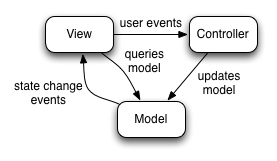
\includegraphics[width=0.85\textwidth]{MVC}
\caption{Modelo-Vista-Controlador (MVC)}
\end{subfigure}
\begin{subfigure}[b]{0.49\textwidth}\centering
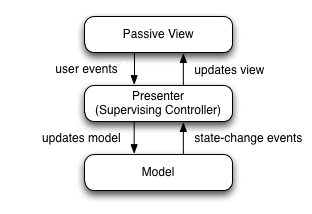
\includegraphics[width=0.94\textwidth]{MVP}
\caption{Modelo-Vista-Presentador (MVP)}
\end{subfigure}
\caption[Patrones MVC y MVP]{Patrones MVC y MVP. La principal diferencia en MVP es que el Modelo no puede interactuar con la Vista si no es a través del Presentador. \\
{\footnotesize \url{http://www.gwtproject.org/articles/testing_methodologies_using_gwt.html}}}
\label{fig:MVP-MVC}
\end{figure}

\section{Arquitectura del sistema}

\section{Clases}

\section{Secuencias}




\resizebox{0.5\textwidth}{!}{\input{diag1.puml}}

\ldots

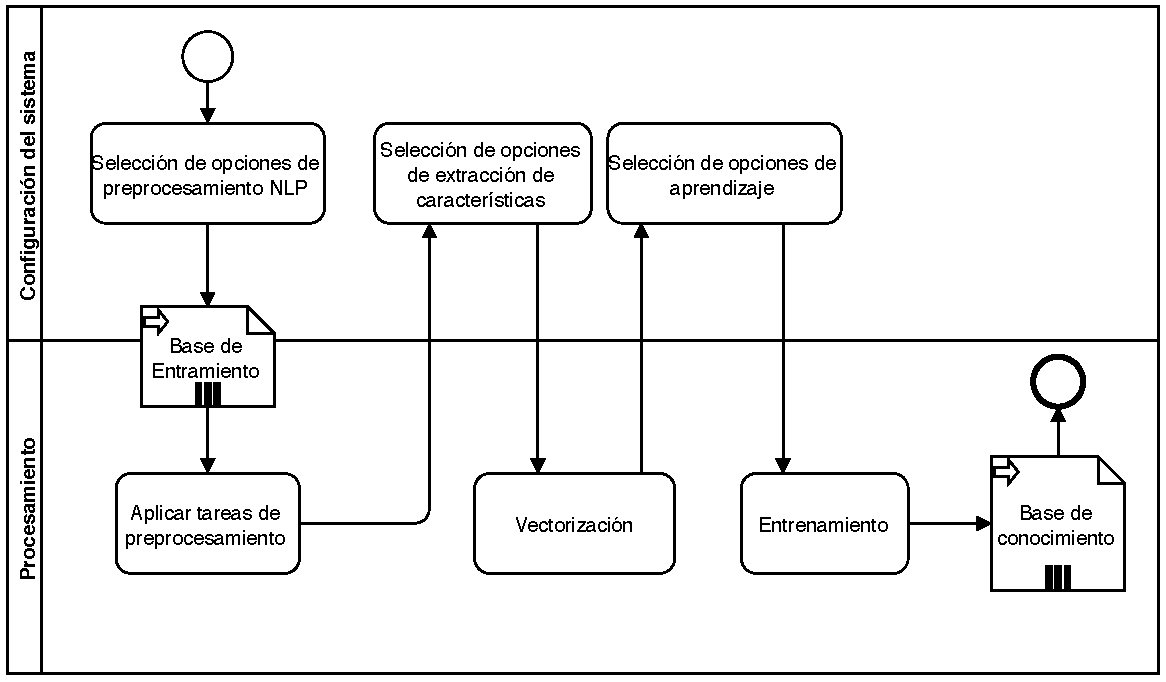
\includegraphics[width=\textwidth]{bpmn-entrenamiento}

\ldots

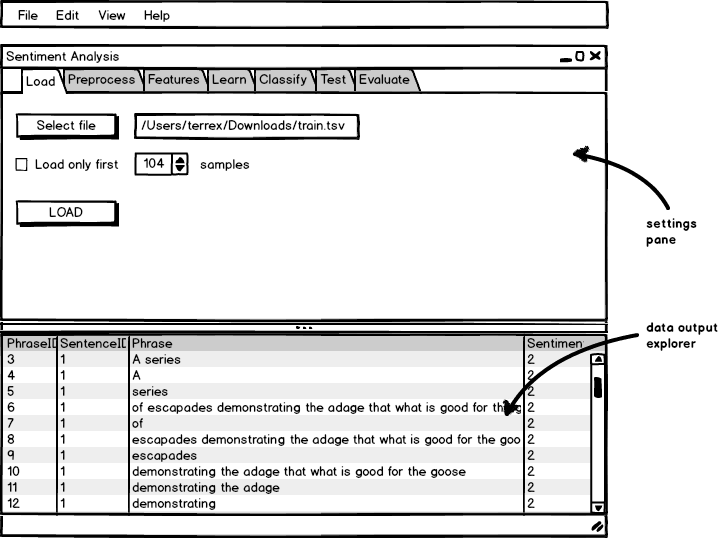
\includegraphics[width=14cm]{gui-1-load}

\ldots

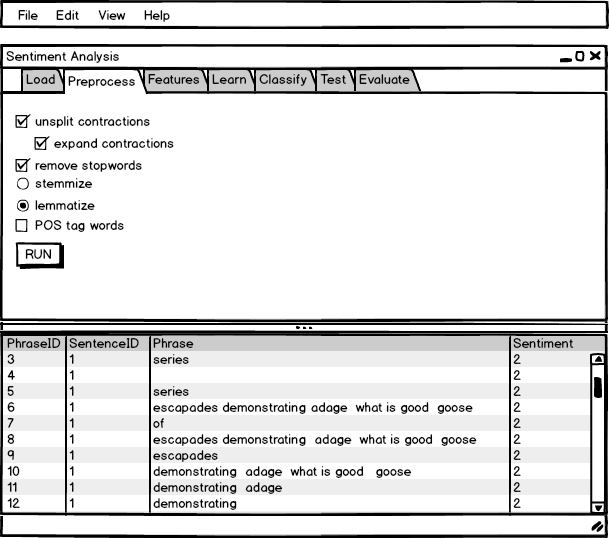
\includegraphics[width=12cm]{gui-2-preprocess}

\ldots

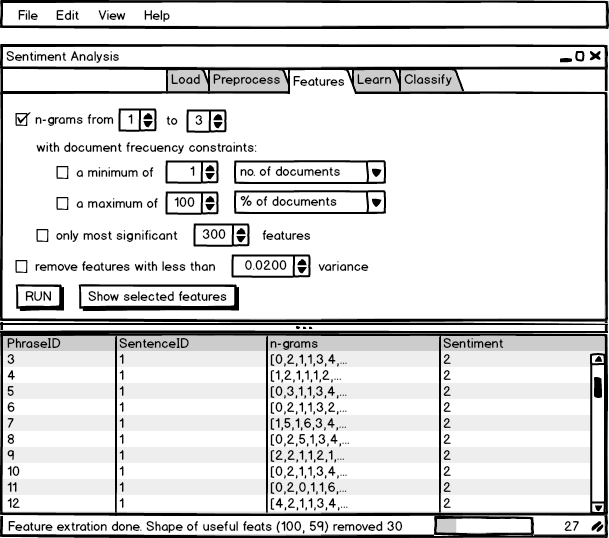
\includegraphics[width=12cm]{gui-3-features}

\ldots

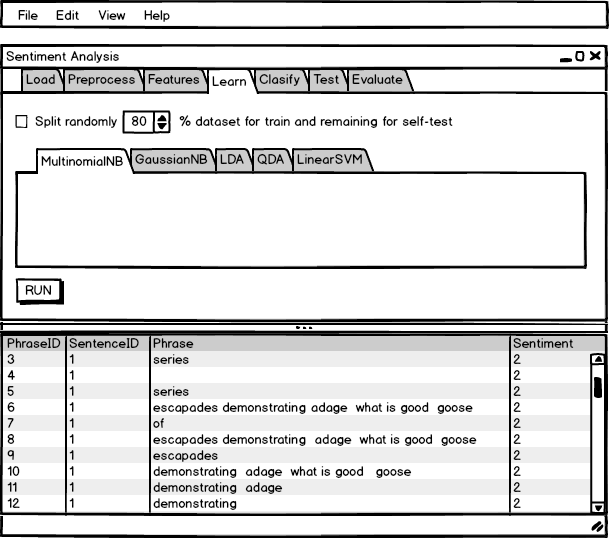
\includegraphics[width=12cm]{gui-4-learn}

\ldots

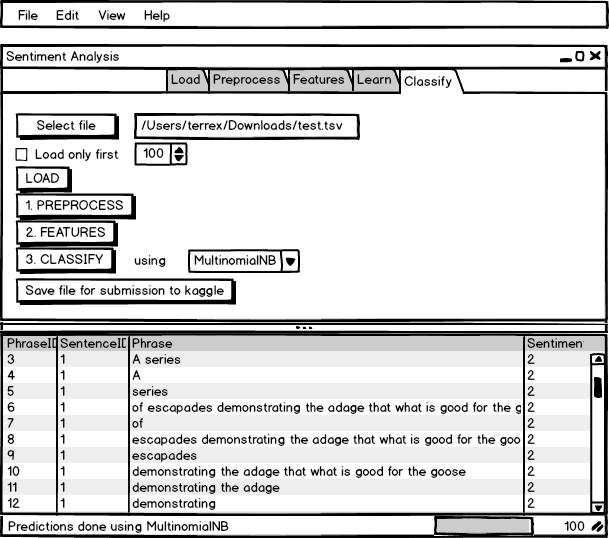
\includegraphics[width=12cm]{gui-5-classify}

\ldots
